\documentclass[../dissertation.tex]{subfiles}

\begin{document}
%%%%% COMPONENTS %%%%%
\section{Components}

% Splitting up the project into multiple components has been useful for
% \begin{itemize}
%   \item Aiding in planning to make the implementation more efficient
%   \item Delegating specific work tasks
%   \item Making the project modular, for example, allowing for a different simulator
%     to be implemented with minimal need to refactor other parts of the codebase
% \end{itemize}

The best way to view the design and implementation of this project is by
splitting up the project into multiple components.
This has been useful for aiding in planning the implementation, as a result
making being efficient with time and requiring less refactoring. The planning
allows for delegating specific work tasks, and making the project modular.
A benefit of making this project modular is improving the maintainability of the
codebase, and allowing for future upgrades or changes, for example, using a different
flight simulator for testing.

\begin{figure}[H]
\centering
  \begin{tikzpicture} [align=center, node distance=4cm]
    \node (connector) [box] {Checklist Tester};
    \node (plugin) [box, right of=connector] {Simulator Connector Plugin};
    \node (formal) [box, left of=connector] {Formal Method};
    \node (simulator) [box, below=0.75cm of plugin] {Flight Simulator};
  
    \draw [<->, arrow] (formal) -- (connector);
    \draw [<->, arrow] (plugin) -- (connector);
    \draw [<->, arrow] (plugin) -- (simulator);
  \end{tikzpicture}
  \caption{Abstract layout of components}
  \label{fig:abstract}
\end{figure}

Each of the components in \autoref{fig:abstract} will be covered in detail in this
chapter.


%%%%% FORMAL METHOD %%%%%
\section{Formal Method}
% \begin{itemize}
%   \item Formal modelling is the heart of the logic for testing checklists
%   \item Formal model created using VDM-SL
%   \item It allows to test that the checklists have been completed properly
%     - and that it is provable
%   \item Model keeps track of
%     \begin{itemize}
%       \item Aircraft state
%       \item Checklist state
%     \end{itemize}
%   \item If an error were to occur in the model, this can be relayed that there was
%     something wrong with running the test for the checklist, such as:
%     \begin{itemize}
%       \item Procedure compromises integrity of aircraft
%       \item There is not enough time to complete the procedure
%       \item There is a contradiction with the steps of the checklist
%     \end{itemize}
% \end{itemize}
Formal modelling is the heart of the logic for testing checklists in this project
and is created using \textit{VDM-SL}.
The formal model is the logic behind the actions of running through a checklist
and checking if the checklist has been completed in the correct manner.

To be able to check that the checklist has been properly completed,
the formal model keeps track of aircraft states, such as what state each switch
in the aircraft is in; and the state of the checklist, such as what steps in the
checklist has been completed.

As there are invariants, pre-, and post-conditions, which are used for setting
well-formedness conditions for types or functions, provide type and input safety,
which will result in an error when broken. This is useful to make sure that
the actions taken when completing the checklist is done correctly, such as making
sure that a switch that may have 3 possible states is moved in properly, such as
moving from off, middle, to on in order, rather than skipping from off to on.
The cases where errors would occur is when these well-formed conditions are broken,
which can be a sign that the checklist has been completed incorrectly, such as
when the checklist is not completed in order, could signify that a step in the checklist
failed, which could mean that the step in the checklist is problematic.

\subsubsection{Testing}
% \begin{itemize}
%   % TODO add references
%   \item Since VDMJ version 4.5, it provides the QuickCheck tool
%   \item This allows for providing counter examples to the model
%   \item The counter examples were helpful to create pre- and post-conditions
%     to avoid any unexpected results from the model
% \end{itemize}

Making sure that the formal model does not have well-formed conditions that can
be broken by the formal model itself is important, as the goal of the formal model
is to have a rigorous specification that is verifiable.

Since \textit{VDMJ} version 4.5.0, the VDM interpreter has included the \textit{QuickCheck} tool,~\cite{vdmj:4.5.0}
which is an automated testing tool to prove and find counter examples to specifications.~\cite{quickcheck}

There were multiple counter examples that was produced by \textit{QuickCheck} that aided
the development of the formal model, as the \lstinline|qc|\footnote{The command to run \textit{QuickCheck} on the formal model in \textit{VDMJ}.}
command in \textit{VDMJ} every time a new function was created to find potential counter
examples and fix them.
Checking every time when creating a new function was useful as it would avoid having to
refactor more of the model.


%%%%% CHECKLIST TESTER %%%%%
\section{Checklist Tester}
The Checklist Tester is what provides a Graphical User Interface (GUI) for defining
checklists to be tested, and to run the tests on the checklist.
It is also responsible for connecting the Formal Method and the Simulator Connector Plugin
together. 

\subsection{Designing}
% \begin{itemize}
%   \item Used Figma to create a design for the application
%   \item Allows for implementing the front end to be faster because:
%     \begin{itemize}
%       \item They act as a requirement for code
%       \item You do not forget what needs to be implemented
%       \item Keeps everything consistent
%       \item Allows to think about making parts of the GUI modular and what components can be reused
%     \end{itemize}
%   \item Figma allows for plugins such as Material 3 colours and Material 3 components
%   \item \autoref{fig:figma-gui} is the final design that will be used for the
%     program
% \end{itemize}

Creating an interface design before creating the GUI is useful as it is a form of
requirements for the code.

\textit{Figma} was used to create the design for the GUI as there is support for plugins
and having a marketplace for components. This saved a lot of time in designing as
Google provides components for \textit{Material 3}%
\footnote{Material 3 is a design system which is used in Compose Multiplatform UI Framework.}
and a plugin for creating a colour scheme for \textit{Material 3}.

Having this design was useful as it aided in understanding
what parts of the GUI could be modular and reused, kept the feel of the
design consistent, and helped memorize what parts of the GUI needed to be implemented.

The final design for the interface can be seen in~\autoref{fig:figma-gui}, where
the components at the top are reusable modules, and the rest below are sections of
the application that the user can navigate through.

\begin{figure}
  \centering
  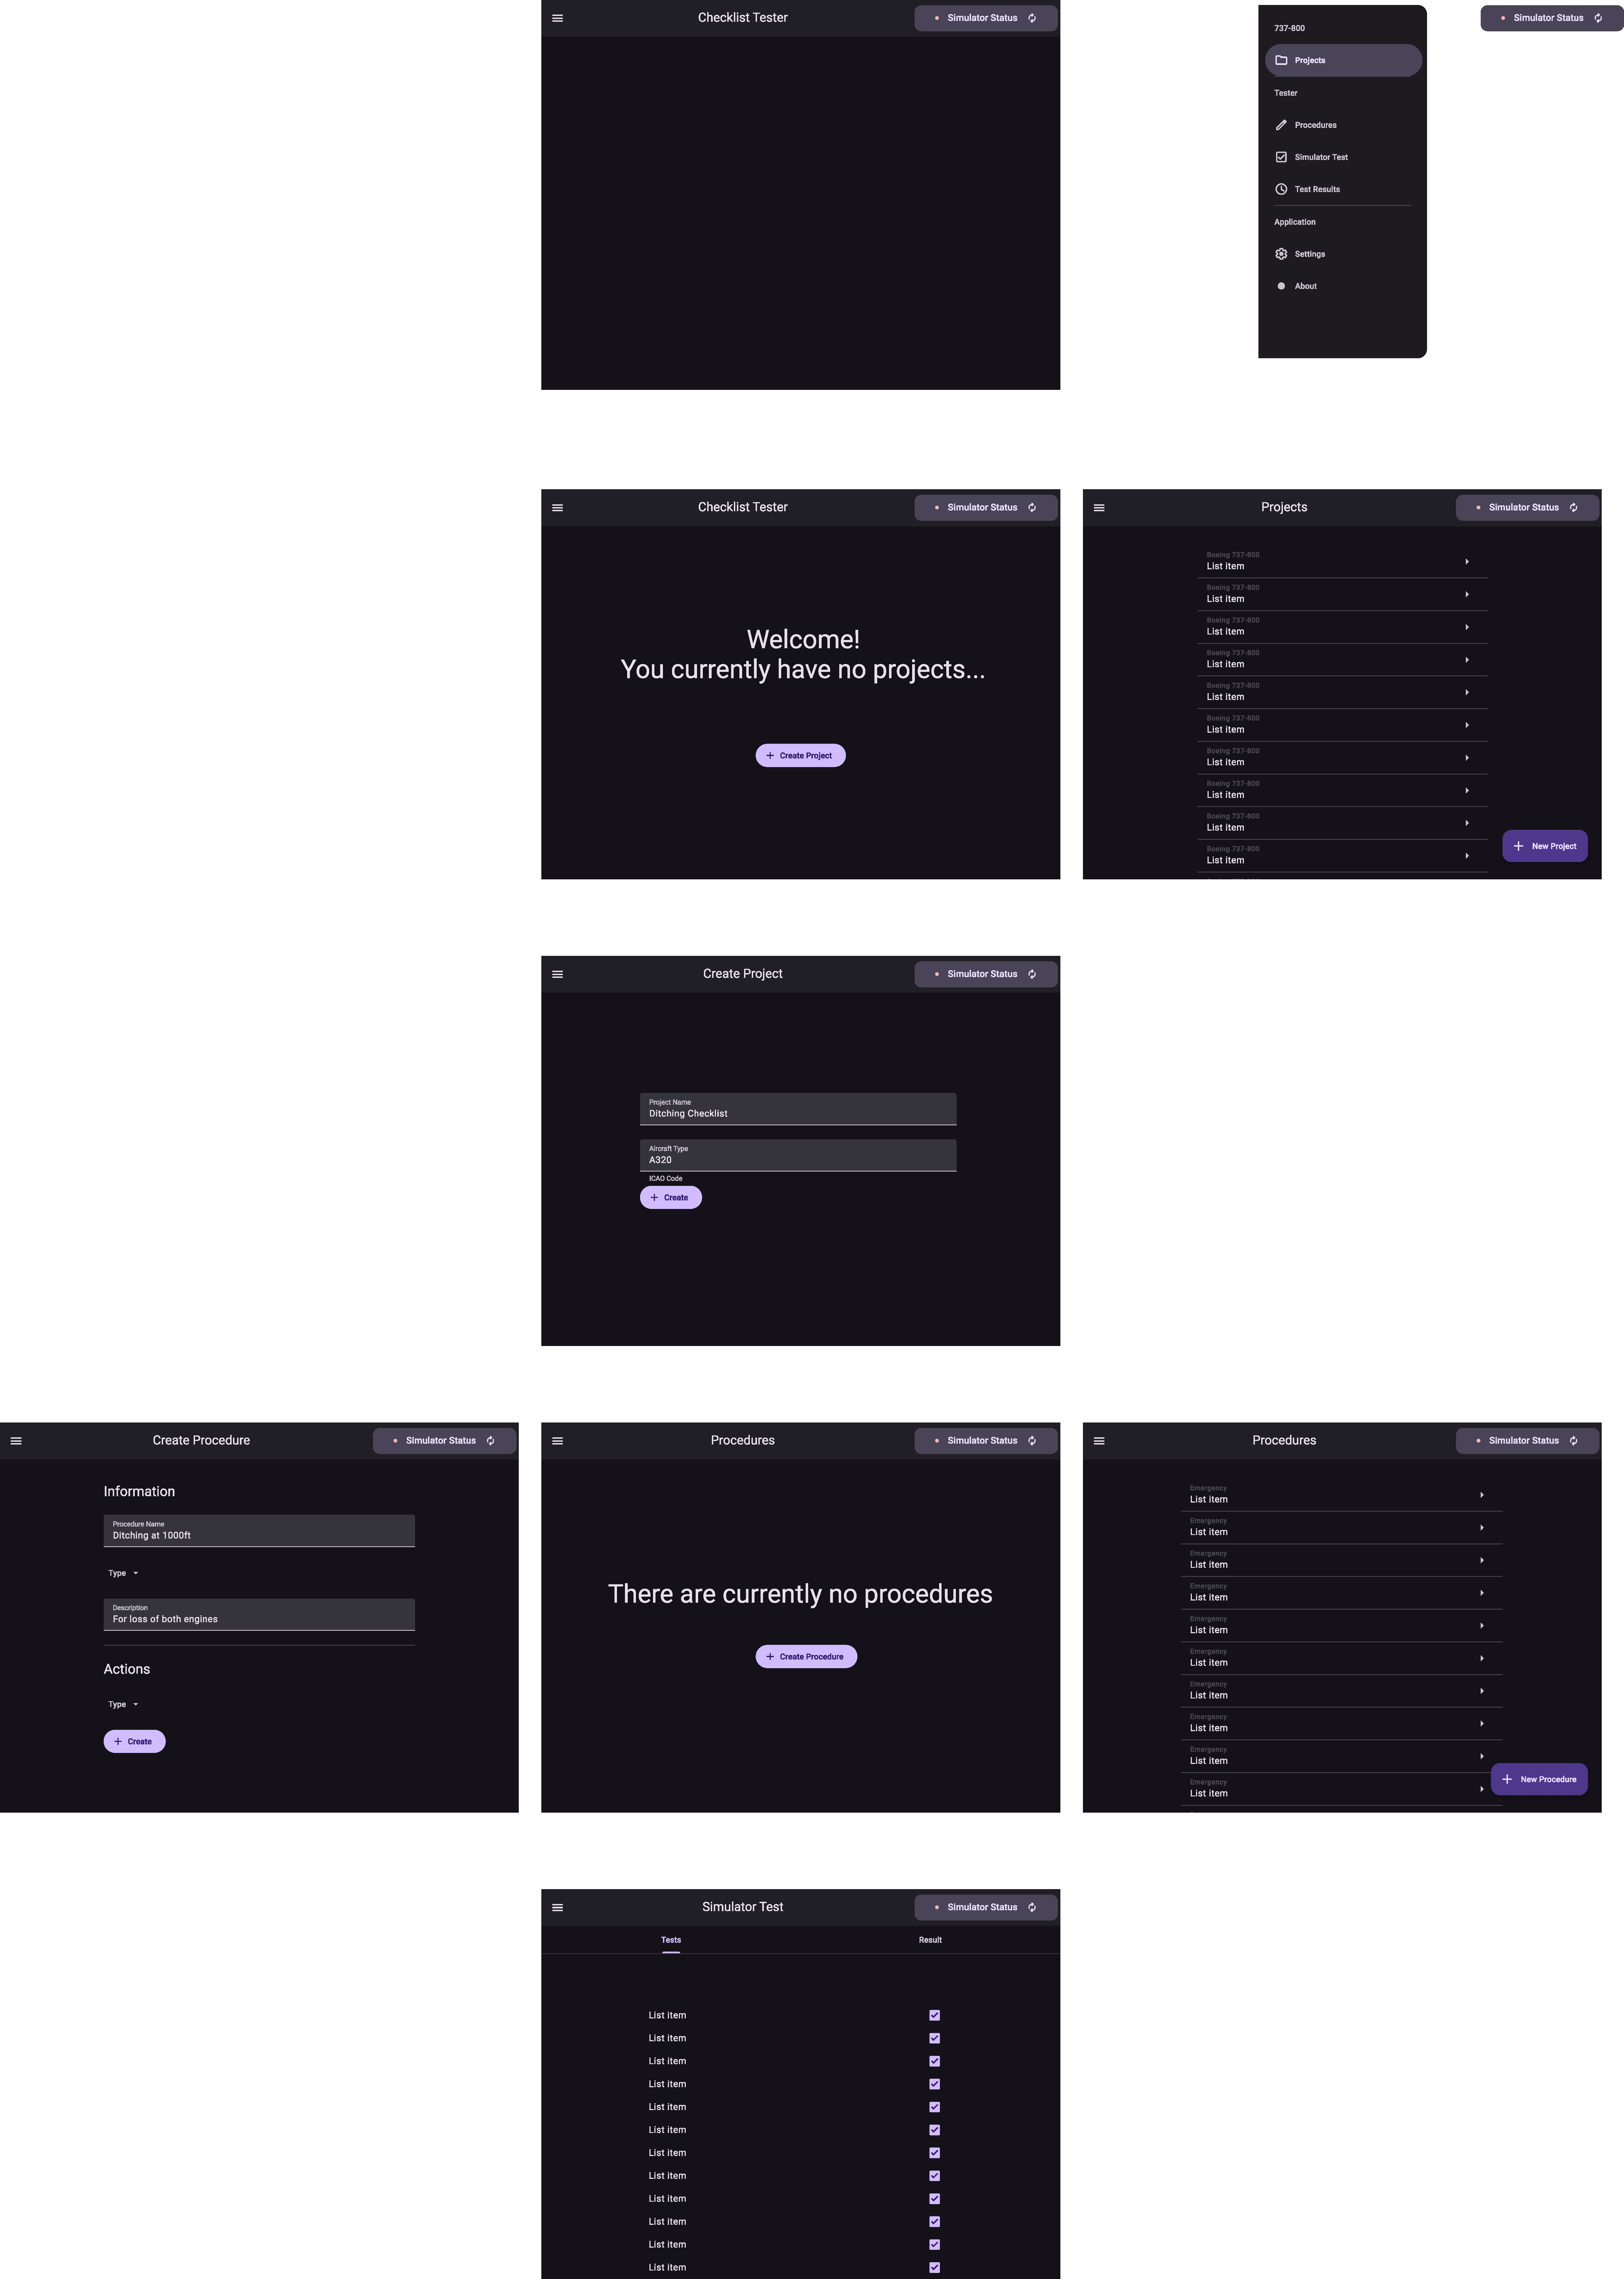
\includegraphics[width=\columnwidth]{images/figma-gui.pdf}
  \caption[GUI in Figma]{Design for the Checklist Connector GUI in Figma}
  \label{fig:figma-gui}
\end{figure}

\subsubsection{Limitations of Figma}
% \begin{itemize}
%   \item The Material 3 Components in Figma do not include features that are available in
%     Jetpack Compose
%   \item In this project, the \enquote{Simulator Test} at the bottom of \autoref{fig:figma-gui}
%     does not include a leading icon~\cite{material:lists}, and therefore had to be a trailing
%     checkbox
%   \item This was overcome by adding comments in Figma as a reminder of how the actual implementation
%     should be like
%   \item Another limitation is that in \autoref{fig:figma-gui}, the title of the screen in the
%     top app bar~\cite{material:top-app-bar} is not centred, and that is because the auto layout
%     feature in Figma allows for equal spacing, rather than having each in a set position
% \end{itemize}

There were some limitations when working with \textit{Figma}, one of them being that
the components created for \textit{Material 3} did not include all the features that are
available in the \textit{Compose Multiplatform} Framework.

This can be seen in the \enquote{Simulator Test} screen at the bottom of~\autoref{fig:figma-gui},
where there is not an option for leading icons~\cite{material:lists} in each of the list items,
and therefore had to be replaced with a trailing checkbox instead. However, \textit{Figma}
allows for comments to be placed on the parts of the design, which was used as a reminder
to use leading icons in the implementation of the design.

Another limitation of \textit{Figma} is that in~\autoref{fig:figma-gui}, the title of the screen
in the top app bar~\cite{material:top-app-bar} is not centred, this is because
the auto layout feature in \textit{Figma} works by having equal spacing between each
object, rather than having each object in a set position. However, this is
not detrimental to the design, it is just obvious that the title is not centred in the
window.


\subsection{Compose Multiplatform}
% \begin{itemize}
%   \item Used the \textit{Kotlin Multiplatform Wizard} to create projects as it allows
%     for runtime environments to be specified (in this case, Desktop and Server)
%   \item Provides necessary build configurations in Gradle
%   \item Planning what to implement important as Compose is designed to use modular
%     components, otherwise a nested mess would occur as Compose is designed to have
%     Composable functions passed in to a Composable function and therefore by design
%     function nests will occur, and the code will be harder to read if not managed correctly.
%     \autoref{list:compose-modular} shows example of using modular code
%     from the Actions screen in project (with code omissions shown in comments)
%   \item Used Voyager~\cite{voyager} to handle screens
%   \item Used Koin~\cite{koin} for dependency injection, to be able to get data from the
%     database and VDMJ
%     \begin{itemize}
%       \item Chose to use it because of Voyager integration with Koin~\cite{voyager:koin}
%       \item Required as the application will be unresponsive when making requests
%         to the database and/or VDMJ
%       \item Used asynchronous coroutines to prevent the program from being blocked
%     \end{itemize}
% \end{itemize}
\subsubsection{Setup}
To set up \textit{Compose Multiplatform}, the \textit{Kotlin Multiplatform Wizard}
was used to create the project as it allows for the runtime environments to be
specified (at the time of creation, Desktop and Server), automatically generating
the \textit{Gradle} build configurations and modules for each runtime environment,
for the specific setup.

\subsubsection{Implementation}
Planning was important when implementing as \textit{Compose} is designed to use modular
components, otherwise a nested mess would occur as \textit{Compose} is designed to
have \textit{Composable}%
\footnote{A \textit{Composable} is a description of the UI that will be built by \textit{Compose Multiplatform}}
objects passed into another \textit{Composable} object.
Therefore, due to how \textit{Kotlin}
is designed with functions, there will be function nesting occurring naturally.
To aid in readability of code due to the nesting functions, the \textit{Composable} objects
are split into separate \textit{Composable} functions.
An example of this is in~\autoref{list:compose-modular}, where instead of
10 \textit{Composable} functions being nested in the \lstinline|Content()| function,
the items in the list (\lstinline|LazyColumn| is used for creating lists) is split
to a separate function, \lstinline|ActionItem()|, as a result making the maximum
amount of nested functions to 5 for all functions.
Another benefit is that it allows for the \lstinline|ActionItem| to be reused
if desired, making the code modular.

Voyager~\cite{voyager} was used to handle the navigation of the application as it
handles replacing previous navigation screens, and allows for inserting data
into the navigation screens.
This is as Voyager has integration with Koin~\cite{koin}\cite{voyager:koin}, which is
a library that specifically handles dependency injection.
Using Koin allowed for data to be fetched from the database and to handle asynchronous
functions, such as running VDMJ and sending instructions to the flight simulator.

\begin{listing}
\inputminted[
  linenos,
  breaklines,
]{kotlin}{code/compose-modular.kt}
\caption[Compose Modular Example]{Example of modular code in Compose}
\label{list:compose-modular}
\end{listing}

\subsection{Storing Data}
% \begin{itemize}
%   \item SQLDelight was used to handle the database by allowing for typesafe Kotlin APIs when interacting with the database.
%     Specifically chosen as it provides support for Compose Multiplatform~\cite{sqldelight}
%   \item It only allows for queries to be written in SQL, which would allow for more complex SQL queries if needed
%   \item SQLite was used for the Relational Database Management System (RDBMS) as it is an embedded database~\cite{sqlite:about},
%     meaning that the database will run in the application, rather than running on a server,
%     either remotely or through local containerization through something like Docker~\cite{docker:container},
%     which could take more time and add complexity as it means implementing additional dependencies
%   \item SQLite also has 100\%~\cite{sqlite:tests} test coverage which is necessary for ensuring that the database will
%     not cause artefacts to the results
% \end{itemize}
\textit{SQLDelight} was used to handle the database as it creates typesafe \textit{Kotlin}
application programming interfaces (APIs) to
communicate to the database.
It was specifically chosen as it provides support for \textit{Compose Multiplatform}~\cite{sqldelight},
making implementing \textit{SQLDelight} into the project easier.

A benefit of using \textit{SQLDelight} is that it only allows for database queries to be
written in SQL, allowing for more complex, and more control of SQL queries. It also
provides 100\% test coverage~\cite{sqlite:tests} which is necessary to ensure that
the database will not cause artefacts to the results.

The choice of relational database management system (RDBMS) to complement \textit{SQLDelight}
was \textit{SQLite} as it allows for the database to run within the application,
rather than running on a separate server, either remotely or through a containerized
instance using something like Docker~\cite{docker:container}. As a result,
this avoided spending extra time implementing the server and
adding extra complexity due to requiring additional dependencies, which would also
add extra maintenance overhead to the project.

\subsubsection{Designing the Database}
% \begin{itemize}
%   \item The database could be thought as having 2 sections
%     \begin{itemize}
%       \item The user inputs to control the tester, i.e. the steps a procedure contains.
%         The tables for these are \textit{Project}, \textit{Procedure}, and \textit{Action}
%       \item The test results for a procedure which are in the \textit{Test}, and \textit{ActionResult} tables
%     \end{itemize}
% \end{itemize}

% \begin{itemize} 
%   \item The design of the database had relationships in mind as the goal was to
%     have a detailed tracking of statistics for each step in the procedure,
%     hence in \autoref{fig:db-erd}
%   \item A \textit{Procedure} can have multiple \textit{Tests}, where each \textit{Test}
%     each contains the result of how each \textit{Action} in \textit{ActionResults}
%   \item The choice of a \textit{Project} was to allow for the segregation of testing
%     different aircraft, as each aircraft has different cockpit layouts
%     and different systems
% \end{itemize}

The database could be looked at as having 2 sections, with relationships in mind
between the two sections, to fulfil of the objectives, as it will allow tracking
of the checklist tests that will be run, as a result being able to provide detailed
statistics of the test. These relationships can be seen in the entity relationship
diagram in~\autoref{fig:db-erd}.

One of the sections is for user inputs to control the tests.
The \textit{Project} table handles creating separate aircraft, or it could be used for
separate iterations of Quick Reference Handbooks (QRHs).
Then the \textit{Procedure} and \textit{Action} table handles defining
steps/actions in a checklist/procedure.

The other section of the database would be providing test results for each of the
checklists, which are stored in the \textit{Test} and \textit{ActionResult} tables.

Expanding on the relationships between each table in~\autoref{fig:db-erd}, the reasons
for these relationships is to allow for segregation of data and the ability to
associate test data with what checklist was tested.
% TODO maybe expand?

\begin{figure}[!htp]
  \centering
  \begin{tikzpicture}[
    auto,
    node distance = 1.5cm
  ]
    % PROCEDURE
    \node[entity] (procedure) {Procedure}
      [grow=up, sibling distance=2.25cm]
      child[grow=down] {node[attribute] {\textbf{id}}}
      child {node[attribute] {name}}
      child {node[attribute] {type}}
      child [grow=north west, level distance=2.15cm]{node[attribute] {description}}
      child [grow=right, level distance=3cm] {node[attribute] {createdUTC}}
      child [grow=left, level distance=3cm] {node[attribute] {modifiedUTC}};

    \node[relationship] (procProj) [above = of procedure] {Contains};

    % PROJECT
    \node[entity] (project) [right = of procProj] {Project}
      [grow=up, sibling distance=2cm]
      child {node[attribute] {name}}
      child {node[attribute] {\textbf{id}}}
      child {node[attribute] {aircraftType}}
      child[grow=right, level distance=3cm] {node[attribute] {createdUTC}}
      child[grow=south east, level distance=3cm] {node[attribute] {modifiedUTC}};

    \node[relationship] (procAct) [below left = of procedure] {Contains};

    % ACTION
    \node[entity] (action) [below left = of procAct] {Action}
      child[grow=up, level distance=2cm] {node[attribute] {step}}
      child[grow=right, level distance=2cm] {node[attribute] {\textbf{id}}}
      child[grow=north west, level distance=2cm] {node[attribute] {type}}
      child[grow=down, level distance=2cm] {node[attribute] {goal}};

    \node[relationship] (actionResult) [below right = of action] {Contains};

    % ACTION RESULT
    \node[entity] (result) [below right = of actionResult] {ActionResult}
      child[grow=up, level distance=2cm] {node[attribute] {\textbf{id}}}
      child[grow=left, level distance=3cm] {node[attribute] {startUTC}}
      child[grow=right, level distance=3cm] {node[attribute] {endUTC}}
      child[grow=south west, level distance=2cm] {node[attribute] {initState}}
      child[grow=south east, level distance=2cm] {node[attribute] {endState}};

    \node[relationship] (testAR) [above right = of result] {Contains};

    % TEST
    \node[relationship] (procTest) [below right = of procedure] {Contains};
 
    \node[entity] (test) [above right = of testAR] {Test}
      child[grow=left, level distance=2cm] {node[attribute] {\textbf{id}}}
      child[grow=north east, level distance=2cm] {node[attribute] {startUTC}}
      child[grow=south east, level distance=2cm] {node[attribute] {endUTC}};

    % RELATIONSHIP PATHS
    \path (procProj) edge node {\(N\)} (procedure)
      edge node {1} (project);

    \path (procTest) edge node {1} (procedure)
      edge node {\(N\)} (test);

    \path (procAct) edge node {1} (procedure)
      edge node {\(N\)} (action);

    \path (actionResult) edge node {1} (action)
      edge node {\(N\)} (result);

    \path (testAR) edge node {1} (test)
      edge node {\(N\)} (result);
  \end{tikzpicture}
  \caption[Connector ER Diagram]{Entity Relationship Diagram for the database in Checklist Connector}
  \label{fig:db-erd}
\end{figure}

\subsubsection{Linking into Compose Multiplatform}
% \begin{itemize}
%   \item Compose Multiplatform has support for different runtime environments,
%     however as this project was only being developed for Desktop, the JVM
%     SQLite driver only had to be considered
%   \item However, the functions for the database were written in the \textit{shared/commonMain}
%     module as there may be a potential for adding Android and iOS support as it may be
%     helpful run the tests on a tablet
%   \item A database transaction had two modules
%     \begin{itemize}
%       \item A class handling SQLDelight API calls only; meaning no conversion of types, which are
%         functions only accessible within module internally, which is located in\\
%         \textit{io.anthonyberg.connector.shared.database}
%       \item SDKs that can handle multiple tables, such as \textit{TestTransaction} which handles database calls
%         when checklists are being tested in the application.
%         And allows for converting types, such as \lstinline|Int| to \lstinline|Long|
%     \end{itemize}
%   \item The separation of these modules was to have in mind unit testing, as
%     it will make it easier to debug if a problem is with SQLDelight transactions
%     are handled, or if there is a conversion error occurring
% \end{itemize}

\textit{Compose Multiplatform} has support for different runtime environments which
should be taken into account when adding \textit{SQLDelight} to \textit{Compose Multiplatform}.
However, as this project is only being developed for Desktop, the \textit{JVM}
\textit{SQLite} driver is the only one necessary to implement.

However, to improve maintainability of the code, the functions of the database was
written in the \lstinline|shared/commonMain| module (a shared module that is accessible
to multiple runtime environments).
This would be useful if there was a need for
adding Android and/or iOS support for this project as some designers may want to
run the tests on a tablet.

Handling the database was done by implementing two modules.
One module is the \lstinline|io.anthonyberg.connector.shared.database| module,
used to handle SQLDelight API calls only; meaning no conversion of types,
functions are only accessible internally within the \lstinline|io.anthonyberg.connector.shared|
module.

The other module is the Software Development Kit (SDK) that handle type conversions,
such as \lstinline|Int| to \lstinline|Long|, and can handle multiple tables,
such as \textit{TestTransaction} SDK that handles calls to multiple tables
when a test is run in the flight simulator.

The separation of these modules was also done to have unit testing in mind because
it will make it easier to debug if a problem is due to how SQLDelight transactions are
handled, or if there are type conversions errors occuring.


\subsection{VDMJ Wrapper}
% \begin{itemize}
%   \item VDMJ is written in Java and it is free open source software that is accessible on
%     GitHub
%   \item This allows for VDMJ to be used as per the licence, GNU General Public License v3
%     (GPLv3)~\cite{vdmj:license}~\cite{gpl3}. This means that as VDMJ is being used as a
%     library, the code for this project has to be licensed with GPLv3 or any GPLv3 compatible
%     licence~\cite{gpl3:library}
% \end{itemize}

VDMJ is written in Java, and it is free open source software that is accessible on GitHub.
This means that VDMJ can be used within any projects as long as the licence is followed.
It is important to follow for ethical and legal reasons, as not following the licensing
would result in breaking copyright law. However, it may not specifically break Newcastle
University's ethics, it would break the ethos behind GPLv3 and free open source software.

The licence VDMJ uses is the GNU General Public License v3 (GPLv3)~\cite{vdmj:license}\cite{gpl3}.
This means that as VDMJ is being used as a library, the code for this project has to be
licensed with GPLv3 or any GPLv3 compatible licence~\cite{gpl3:library}.

\subsubsection{Implementing VDMJ}
% \begin{itemize}
%   \item VDMJ has packages available on Maven Central making adding it as a dependency simple
%   \item The package used was \lstinline|dk.au.ece.vdmj:vdmj| with version \lstinline|4.5.0|
%   \item However, initially when implementing VDMJ, \lstinline|4.5.0-P| was used accidentally,
%     and it led to debugging why imports were not working; and therefore the \lstinline|-P|
%     versions are not suitable
%   \item The initial method of implementation was using a Ktor server that would have run
%     alongside the desktop application, where the server would handle Representational State Transfer (REST)
%     API calls
%   \item This was unnecessary as the \textit{interactive} mode of VDMJ was able to run on
%     the desktop application itself. However, the Ktor was useful for debugging and testing as
%     an API route was created to allow VDMJ commands to be executed through a URL

%   \item To be able to get the outputs from VDMJ, a \lstinline|ConsolePrintWriter| new had to be
%     created from the \lstinline|com.fujitsu.vdmj.messages| package; which handles writing to
%     the console \textit{stdout}. This then gets used to replace the \lstinline|Console.out| and
%     \lstinline|Console.err| in the \lstinline|com.fujitsu.vdmj.messages| package

%   \item Parsing commands into VDMJ interface - was more difficult
%     \footnote{The objects created here are provided by the \lstinline|java.io| package.}
%   \begin{itemize}
%     \item Created a \lstinline|PipedInputStream| object, that gets connected to a \lstinline|PipedOutputStream|
%       object by passing the latter object in as a parameter. The \lstinline|PipedOutputStream| is then used
%       to pass inputs into \lstinline|PipedInputStream|
%     \item To be able to write to this stream, a \lstinline|BufferedWriter| is created by passing the \lstinline|PipedOutputStream|
%       with a bridge \lstinline|OutputStreamWriter| that encodes characters into bytes
%     \item For VDMJ to be able to read the input stream, a separate object had to be created, \lstinline|BufferedReader|,
%       where the \lstinline|PipedInputStream| gets parsed through a bridge, \lstinline|InputStreamReader| that converts
%       bytes to characters
%       % TODO create a diagram of this (better than having code)
%       % BufferedWriter -> encode to byte -> Stream -> decode to char -> VDMJ
%   \end{itemize}
% \end{itemize}

\textit{VDMJ} has packages available on Maven Central%
\footnote{Maven Central is a repository that stores dependencies required to build
projects}
making adding it as a dependency simple as it would require to be specified within
the \textit{Gradle} build configurations.
The package used was \lstinline|dk.au.ece.vdmj:vdmj| with version \lstinline|4.5.0|,
however, initially when implementing VDMJ, \lstinline|4.5.0-P| was used accidentally,
and it led to the rabbit hole of debugging why imports were not working, and it was
found that the \lstinline|-P| versions of VDMJ is not suitable to be used when being
implemented intentionally a project.

The initial method of implementation was to use a Ktor server that would run
alongside the desktop application, where communication between the desktop application
and the server would be handled through Representational State Transfer (REST) API calls.
However, this was unnecessary as the \textit{interactive} mode of \textit{VDMJ}
was able to run on the desktop application itself. But using Ktor was useful for
debugging and testing using as \textit{VDMJ} commands could be run through an
API route.

The major hurdle within implementing \textit{VDMJ} as a wrapper was fetching the
outputs that \textit{VDMJ} sends to the console. This was implemented by
creating a new \textit{VDMJ} console handler \\\lstinline|ConsolePrintWriter|, that
handles writing to \textit{stdout},
which is from the \lstinline|com.fujitsu.vdmj.messages| package.
This then gets used to replace the \lstinline|Console.out| and
\lstinline|Console.err|, from the same \textit{VDMJ} package, which
will store the outputs to the console into a variable instead.

Parsing commands into the \textit{VDMJ} interface was more difficult as it required
using Java functions\footnote{The objects created here are provided by the \lstinline|java.io| package.}
to act as if the program wrote something directly into the \textit{VDMJ} interactive console.
\autoref{fig:vdmj-io} shows a simplified flowchart of how inputs are handled.
A \lstinline|PipedInputStream| object was created, that gets connected to a
\lstinline|PipedOutputStream| object by passing the latter object in as a parameter.
The \lstinline|PipedOutputStream| is then used to pass inputs into \lstinline|PipedInputStream|.
The \lstinline|PipedInputStream| handles sending inputs to the \textit{VDMJ} console.
However, to be able to write to these streams, a \lstinline|BufferedWriter|,
which is used to send inputs, is created by
passing the \lstinline|PipedOutputStream| with a bridge \lstinline|OutputStreamWriter|
that encodes characters into bytes.
For \textit{VDMJ} to be able to read the input streams, the \lstinline|PipedInputStream|
gets parsed through a bridge, \lstinline|InputStreamReader| that converts
bytes to characters, and then allows \textit{VDMJ} read these characters through
a \lstinline|BufferedReader|.


\begin{figure}[!htp]
  \begin{tikzpicture}[node distance=2cm, align=center]
    \node (write) [box] {Run VDM command};
    \node (buffWrite) [box, below of=write] {BufferedWriter};
    \node (outputStream) [box, below of=buffWrite] {Encode to byte};
    \node (pOutputStream) [box, below of=outputStream] {PipedOutputStream};
    \node (pInputStream) [box, right of=pOutputStream, xshift=3cm] {PipedInputStream};
    \node (inputStream) [box, above of=pInputStream] {Decode to charset};
    \node (buffRead) [box, above of=inputStream] {BufferedReader};
    \node (vdmj) [box, above of=buffRead] {Read by VDMJ};

    \draw[->, arrow] (write) -- (buffWrite);
    \draw[->, arrow] (buffWrite) -- (outputStream);
    \draw[->, arrow] (outputStream) -- (pOutputStream);
    \draw[<->, arrow] (pOutputStream) -- (pInputStream);
    \draw[->, arrow] (pInputStream) -- (inputStream);
    \draw[->, arrow] (inputStream) -- (buffRead);
    \draw[->, arrow] (buffRead) -- (vdmj);
  \end{tikzpicture}
  \centering
  \caption[VDMJ IO Stream]{Flowchart of VDMJ Input/Output Stream handling}
  \label{fig:vdmj-io}
\end{figure}


\subsubsection{Handling VDMJ Command Outputs}
% \begin{itemize}
%   \item VDMJ outputs are handled using string manipulation
%   \item Created into objects that are replicas of types in VDM-SL
%   \item The string manipulation allows specifying where the outputs
%     of the object go
% \end{itemize}
When running a command in the \textit{VDMJ}, it will produce an output
as a string for the returned variable in the function that was executed.

To handle these strings, \textit{Kotlin} string manipulation was used,
similar concept to \textit{Regex},
to decode the string and convert the string into correct types and store them
in specific types in the formal specification, recreated in \textit{Kotlin}.

The types recreated from the formal specification were the records types.
This was done by using \textit{Kotlin} data classes,
which had functions implemented with the purpose of convert the stored types in \textit{Kotlin}
to an identical \textit{VDM-SL} representation of the values in that type.



% Talk about how XPC was used here, not how it was implemented
\subsection{Connecting to the Flight Simulator}
% \begin{itemize}
%   \item Implemented XPC into the flight simulator
%   \item Allowed being able to
%   \begin{itemize}
%     \item Read data from the simulator
%     \item Override dataref variables in the simulator
%     \item Execute other commands that can manipulate certain switches
%       where otherwise unable to by changing the value of the dataref
%   \end{itemize}
%   \item Made sure to check that the simulator is connected before running
%     the test to avoid exceptions being thrown
%   \item Logic behind doing an action is to fetch the action's initial state
%     from the dataref variable name, run the action, then get the final state
%     of the dataref
%   \item There is an artificial delay added before running the action to
%     try and simulate a delay of the crew's lag between reading the step of the
%     checklist and doing the action
%   \item Because of this, XPC had to be run asynchronously to prevent the
%     GUI from hanging as a function is waiting to complete - prevents misleading
%     user that the application has crashed, and it looks better 
% \end{itemize}

X-Plane Connect (XPC) was used to connect the desktop application to the flight simulator.
X-Plane stores values of the aircraft states in what they call \enquote{datarefs}.
XPC allows to use these datarefs in external programs through libraries that complement the
plugin used in X-Plane. The features that XPC brings is the ability to read data from the
simulator, override dataref values, and execute other commands that can manipulate
certain switches of the aircraft, where otherwise unable to by changing the value of the
dataref.

Before running commands through XPC in the Checklist Tester, a check was run to verify
that the X-Plane was running to avoid exceptions being thrown by XPC if it was not able
to connect to the flight simulator.

When running the tests, each step in the checklist (referred to as \enquote{action} in 
the logic implemented with XPC below) would go through an order with XPC.
The first step is to fetch the initial state of the action in the simulator.
Then, artificial delay is added before doing the
action in the flight simulator, to imitate delay of the crew's lag between reading the step of
the checklist and doing the action. Finally, XPC will execute the action in the flight simulator
and get the final state of the action's sate in the flight simulator.
Then in the Checklist Tester, it checks if the goal of the action was achieved in the final
state.

Whilst running these actions in XPC, the initial state and time, and final state and time
is recorded on the database to be used for the results of the test. These actions of
running the XPC commands and storing the data on a database is run asynchronously to prevent
the GUI from freezing as the application is waiting for a function to complete. This avoids
misleading the user that the application has crashed, whilst allowing for test running animations
within the GUI to continue being shown, making it look nicer.


\subsection{Testing}
% \begin{itemize}
%   \item Testing can be run with Gradle when it comes to running unit tests
%   \item Decided to use JUnit 5 as it provides additional tools such as
%     statistics, integration with IntelliJ to view code coverage,
%     or being run in continuous integration tests
%   \item The testable components in this project is mostly backend modules as
%     the GUI made in Compose is not the focus of the project, and it would
%     require a lot of extra time
%   \item Unit tests have been made for the database and Koin
%   \item Koin comes with tests that can be automatically be generated
%   \item Ethos when testing was to try and find exploits, act as a
%     user who may mishandle inputs, and stress testing functions
%     by passing parameter with hundreds of objects
% \end{itemize}
\textit{Gradle} provides testing integration, which allows for unit tests to
be run through \textit{Gradle}, with a command, in GitHub Continuous Integration for
commits and packaging, or before building a complied application.

\textit{JUnit} 5 was used for testing as other development tools provide integration with
\textit{JUnit}, such as integration with IntelliJ to view code coverage.

The testable components in this project are mostly backend modules as the
GUI is difficult to write unit tests for there are not a lot of tools
for testing \textit{Compose} components, and testing the GUI would be an
inefficient use of time as it is not the focus of this project.

For the backend, unit tests were written for the database and
the dependency injection.
Koin provides tools that allow unit tests to be
automatically generated, as a result meaning it was worth the time to implement
tests for dependency injection.
The ethos when writing unit tests was to try and find exploits, act as a user who
may mishandle inputs, and stress test functions that were developed.


\subsubsection{Testing for Resource Usage}
% \begin{itemize}
%   \item The application was tested using the \textit{Profiler} tool on
%     IntelliJ IDEA 2024 (Ultimate Edition) to find potential
%     memory leaks
%   \item One problem found was the initial VDMJ wrapper which would use the execute
%     command instead of the interpreter, which would require reinitializing
%     the entirety of VDMJ, which resulted in a slight memory leak and a
%     massive write usage
% \end{itemize}

The application was tested using the \textit{Profiler} tool provided by
IntelliJ IDEA 2024 (Ultimate Edition) to find potential memory leaks and
CPU intensive functions.

One problem was found which was the initial versions of the \textit{VDMJ} wrapper that was
created. The initial version did not use interactive mode, which resulted in
\textit{VDMJ} reinitializing each time a command was executed, resulting in a slight
memory leak and a massive memory write usage.



%%%%% Simulator Connector Plugin %%%%%
\section{Simulator Connector Plugin}
% Talk about creating your own (originally happened) vs using something else that was developed
% Maybe talk about original plan? i.e. <project root>/plugin


\subsection{Creating Maven Package}
% Gradle
% Testing
% GitHub CI
% \begin{itemize}
%   \item XPC package is not published on a public Maven repository
%   \item There has been a pull request that was merged to the \textit{develop} branch
%     that provides Maven POMs~\cite{xpc:pom}. However, the maintainer for the
%     project, at the time, did not have enough time to figure out the process of
%     publishing the package to a Maven repository~\cite{xpc:pom-time}
%   \item Therefore, had to find an alternative way to implement
%   \item Jitpack~\cite{jitpack}
%   \begin{itemize}
%     \item In theory, simple to publish a repository, all that is required is a GitHub
%       repository and searching if one has already been created on JitPack or build and publish
%       a specific version
%     \item However, due to the structure of the XPC repository, JitPack could not locate the
%       build tools (Apache Maven in this case) as JitPack only searches on the root directory
%       for the compatible build tools
%   \end{itemize}
%   \item Gradle gitRepository~\cite{gradle:gitRepository}
%   \begin{itemize}
%     \item There was not a lot of documentation
%     \item Ambiguous on how to define directory for where the Java library is located in the Git repository
%     \item However, as XPC was only built with Maven, Gradle was not able to add the dependency as \lstinline|gitRepository()|
%       only works with Gradle builds~\cite{gradle:gitRepoGradleOnly}
%   \end{itemize}
% \item Resorted to using a compiled Jar file and adding the dependency to Gradle
% \item Not happy about that because it means maintaining it will be more difficult as
%   it is not as simple as just changing the version number
% \item Later, resorted to adding Gradle build files to XPC
% \item Used automatic conversion from Maven to Gradle using \lstinline|gradle init| command~\cite{gradle:migratePOM}
% \item Had to add local dependencies due to how Gradle works differently
% \item Had to fix previous structure of Maven POM as the grouping as not good
% \end{itemize}

The XPC Java library is not published on a public Maven repository. There has been a pull
request that was merged into the \textit{develop} branch that provides Maven POMs~\cite{xpc:pom}.
However, the maintainer of the project, at the time, did not have enough time to figure out
the process of publishing the package to a Maven repository~\cite{xpc:pom-time}.

Therefore, an alternative had to be found to implement the XPC library and there were
a few attempts made, before remaking the build files and publishing the library onto
GitHub's Maven repository.

The first tool found was Jitpack~\cite{jitpack}, which in theory makes it simple to
publish to their own public Maven repository, as the requirements to publish the package
was to input a desired GitHub repository and search if one has already been created on
JitPack. If it has not been, JitPack will build and publish a desired version of
the project. However, due to the structure of the XPC repository, JitPack was unable to
locate the build tools (Apache Maven in this case) as JitPack only searches the root directory
of the repository for the compatible build tools; XPC's build tools was in the \lstinline|Java/|
directory.

The next step was to look if Gradle was able to handle building and implementing libraries
from a GitHub repository, to which there is the \lstinline|gitRepository| function~\cite{gradle:gitRepository}.
It was a bit problematic trying to figure out how the \lstinline|gitRepository| function worked
as there is not a lot of documentation provided for it, and the documentation provided was
ambiguous on how to define the directory where the Java library is located in the Git
repository. However, as XPC was only built with Maven, Gradle was unable to add the dependency
to the project as \lstinline|gitRepository| only works with Gradle builds~\cite{gradle:gitRepoGradleOnly}.

Therefore, as a temporary solution, implementing the library was resorted to using the Jar
files provided with XPC and adding the dependency to Gradle. But this caused future maintainability
problems as updating the XPC library would require downloading the Jar file manually and replacing
the previous version. It also results in other tools being unable to check if there is a new
version of XPC available.

This temporary solution was later fixed by creating a fork of XPC and implementing 
\textit{Gradle} build files.
As there already are \textit{Apache Maven} build files for the Java library,
the \lstinline|gradle init| command could be used to automatically generate
\textit{Gradle} build files based on the \textit{Apache Maven} build files~\cite{gradle:migratePOM}.
There was still some configuration required for the \textit{Gradle}
build files as the previous \textit{Apache Maven} configuration was not
properly implemented, resulting in fixing local dependencies and splitting up the
library into their respective package groups.


\subsubsection{Continuous Deployment of the Maven Package}
% \begin{itemize}
%   \item Used GitHub's template for Gradle package publishing
%   \item Required some setup in Gradle build files
% \end{itemize}

To be able to use the new package created with \textit{Gradle} and publish them,
GitHub provides tools to publish \textit{Gradle} projects automatically.
This required defining in the build files on where \textit{Gradle} can
publish the packages.
This was combined GitHub's Gradle Continuous Deployment template
to publish the package, with the only change to the template being defining the working
directory to be the \lstinline|Java/|



%%%%% SCENARIOS %%%%%
\section{Scenarios}
% \begin{itemize}
%   \item Use a Quick Reference Handbook (QRH) to find potential list of checklists to test
%   % TODO find these accident reports
%   \item Look at previous accident reports that had an incident related to checklists
%     and test it with my tool to see if it will pick it up
%   \item These previous accident reports can be good metrics to know what statistics to
%     look out for
% \end{itemize}
To be able to test if the objectives were met, QRHs can be used to find a potential
list of checklists to test for.
This can also be done by looking at previous accident reports that had incidents related
to checklist as they provide problems related to the checklist,
for example the US Airways Flight 1549 accident report includes the checklist
used in the appendix~\cite{ntsb:AWE1549}.
With these checklists, they can be implemented to the Checklist Tester tool
see if it will detect problems within the checklist. 

\end{document}
